\chapter{Alternative Measures of Clearance Time}\label{ch:alternative}

\section{Alternative endpoints}
\subsection{PC50}
PC50 was estimated by log-linear interpolation. The PC50 clearance times thus obtained are plotted in Figure \ref{pc50anova} by experimental factors with sub-plots to look for interactions.
\begin{figure}[p]
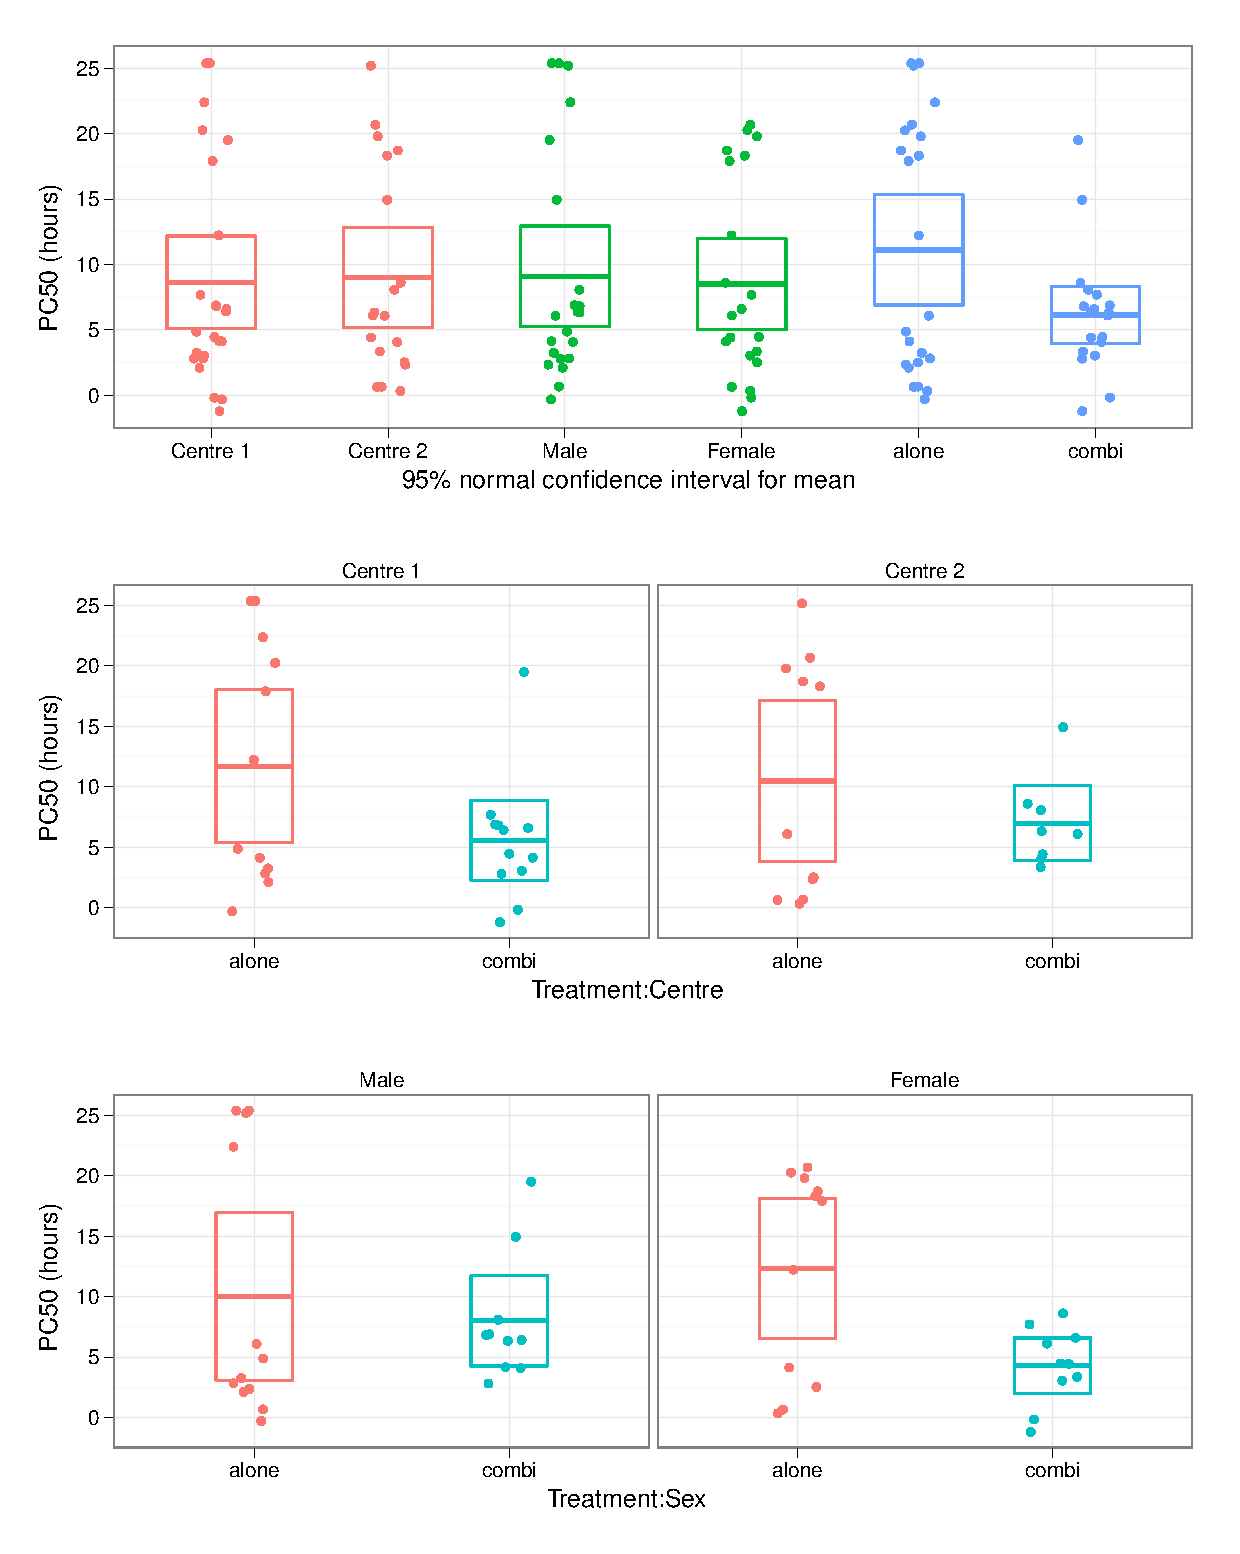
\includegraphics[width=150mm]{pc50anova.eps} 
\caption{Comparison of PC50 main effects and interactions with $t$ distribution 95\% confidence intervals for the means}
\label{pc50anova}
\end{figure}
A similar pattern can be seen as for PC90 (Figures \ref{pc90boxes} and \ref{pc90interaction} on pages \pageref{pc90boxes} and \pageref{pc90interaction}). The same key features are present namely
\begin{itemize}
\item No difference between centres.
\item A reduction in clearance time with the combined treatment, but only for female subjects.
\item A greater variance for subjects on the single (``alone'') treatment.
\end{itemize}

The same procedure of inspecting the distribution of standardized residuals was followed for choosing an appropriate ANOVA model for the data. As with PC90 it was found that the most suitable model for the PC50 clearance time was a 2-way ANOVA model by sex and treatment with a square-root transformation of the dependent variable, fitted by weighted least-squares, using the variances of the two treatment groups as the weighting. The results are shown in Table \ref{aov50}.
%> summary(PC50.loglin2rwt.aov)
%              Df Sum Sq Mean Sq F value  Pr(>F)  
%Sex            1  1.104   1.104  1.1652 0.28702  
%Treatment      1  2.089   2.089  2.2055 0.14556  
%Sex:Treatment  1  3.010   3.010  3.1771 0.08246 .
%Residuals     39 36.949   0.947
\begin{table}[h]
\centering
\caption{ANOVA table for PC50 model}\label{aov50}
\begin{tabular}{l|rrrrrl}
Source&Sum Sq.&df&Mean Sq.&$F$&P($>F$)\\
\hline
$Sex$				& 1.10 & 1 & 1.10 & 1.17 & 0.287 & \\
$Treatment$			& 2.09   & 1 & 2.09   & 2.21   & 0.146 & \\
$Sex\times Treatment$	& 3.01   & 1 & 3.01   & 3.18   & 0.082 & \\
$Residuals$			& 36.95 & 39 & 0.947 &&&\\
\hline
Total&43.15&42&&&
\end{tabular}
\end{table}

Although Figure \ref{pc50anova} seems to show a sex-treatment interaction effect on clearance times we do not have evidence at the 5\% level to reject the hypothesis that there is no effect of sex or treatment. This is probably because the difference between clearance times is smaller than for PC90 and we don't have enough data to detect this difference at the 5\% level.

The mean PC50 clearance times and confidence intervals are shown in Table \ref{inference50}.
\begin{table}[h]
\centering
\caption{Mean PC50 clearance times by sex and treatment}\label{inference50}
\begin{tabular}{|l|c|c|}
\hline
&Clearance time PC50&95\% conf. int.\\
Factor levels&(hrs:mins)&(hrs:mins)\\
\hline
Male, single treatment 		& 6:47 & (2:37, 12:54) \\
Female, single treatment		& 10:02 & (4:34,  17:37) \\
Male, combined treatment	& 7:22 & (3:50, 12:03) \\
Female, combined treatment	& 2:54 & (0:54, 6:03) \\
\hline
\end{tabular}
\end{table}

For female subjects the mean decrease in PC50 in the combined treatment group over the single treatment group is 7.1 hours with a 95\% confidence interval of (0.7, 9.9) hours.

\subsection{PC99}
%The log-linear interpolated PC99 values are plotted in Figure \ref{pc99anova}.
%\begin{figure}[p]
%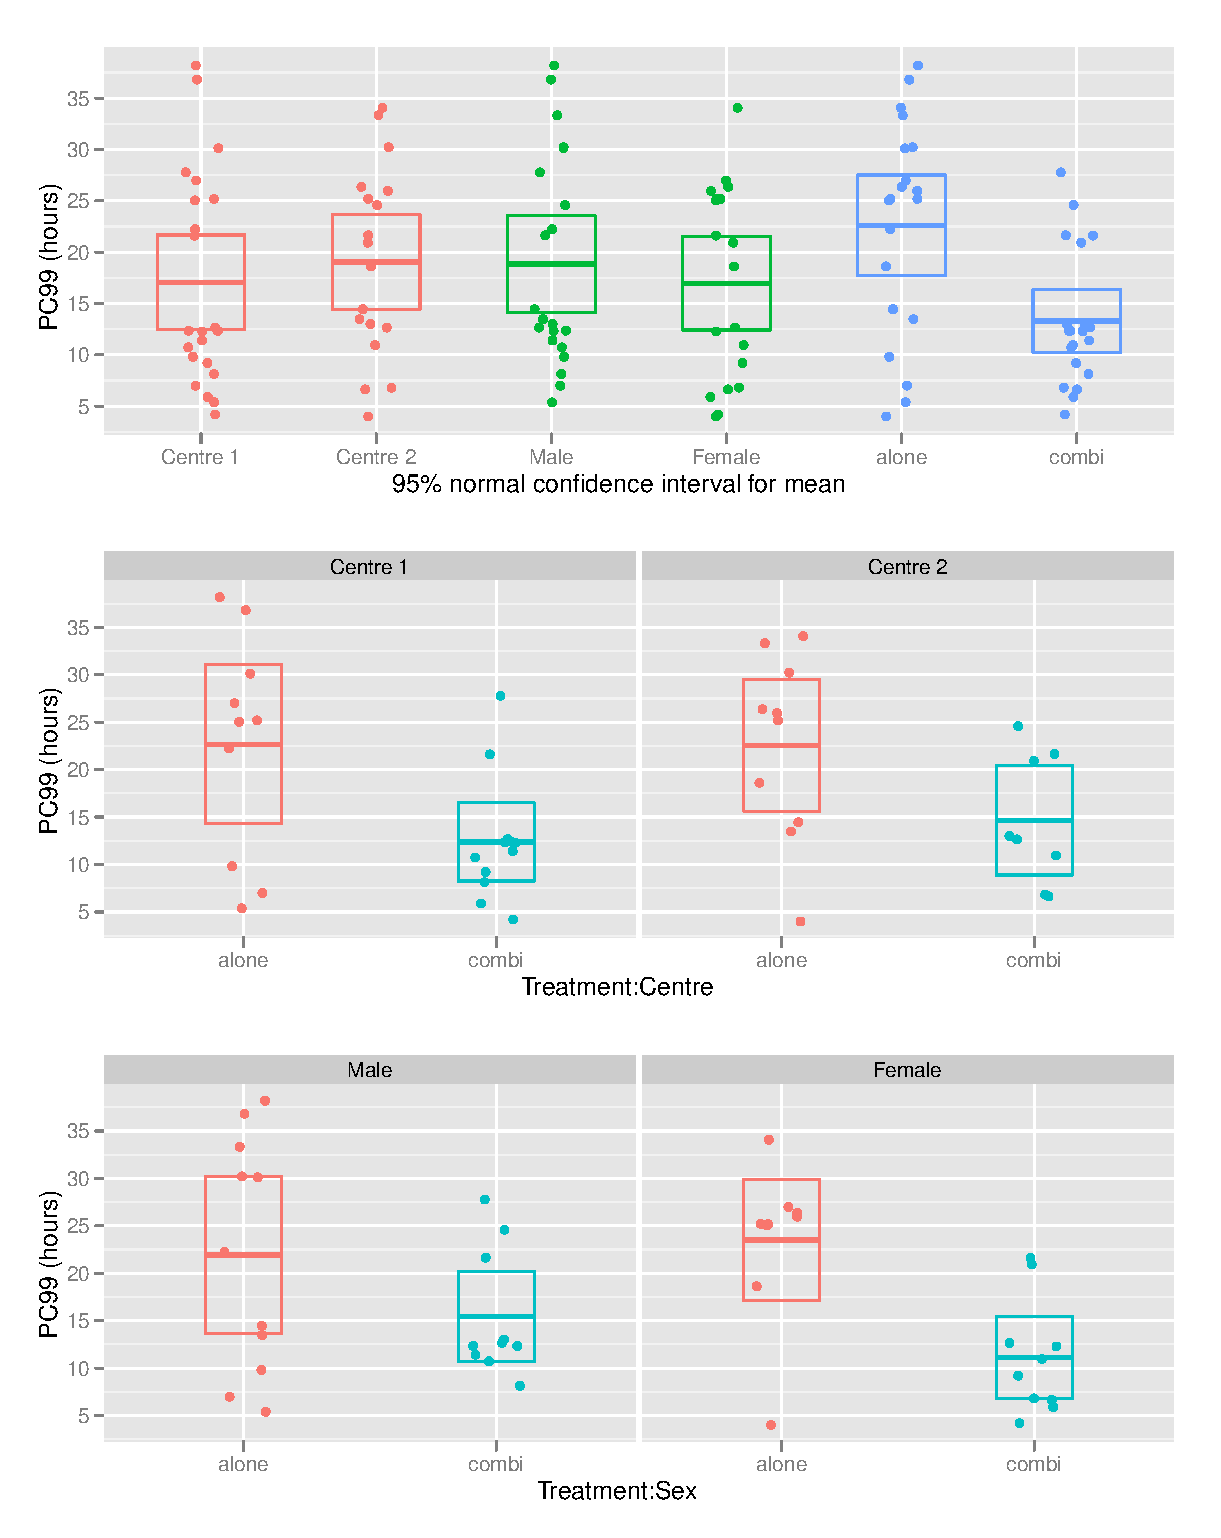
\includegraphics[width=150mm]{pc99anova.eps} 
%\caption{Comparison of PC99 main effects and interactions with $t$ distribution 95\% confidence intervals for the means}
%\label{pc99anova}
%\end{figure}
For 3 subjects the parasite count did not reach the PC99 level by the end of the study. Rather than simply omit these subjects and thereby bias the comparison - as these 3 subjects are ones with long clearance times on the single treatment - we can make estimates of the possible range of PC99 for these subjects had data been taken for a longer time period. In order to do this we make a linear extrapolation to the PC99 level as shown in Figure \ref{pc99extrap} for subjects 285 and 98.
\begin{figure}[h]
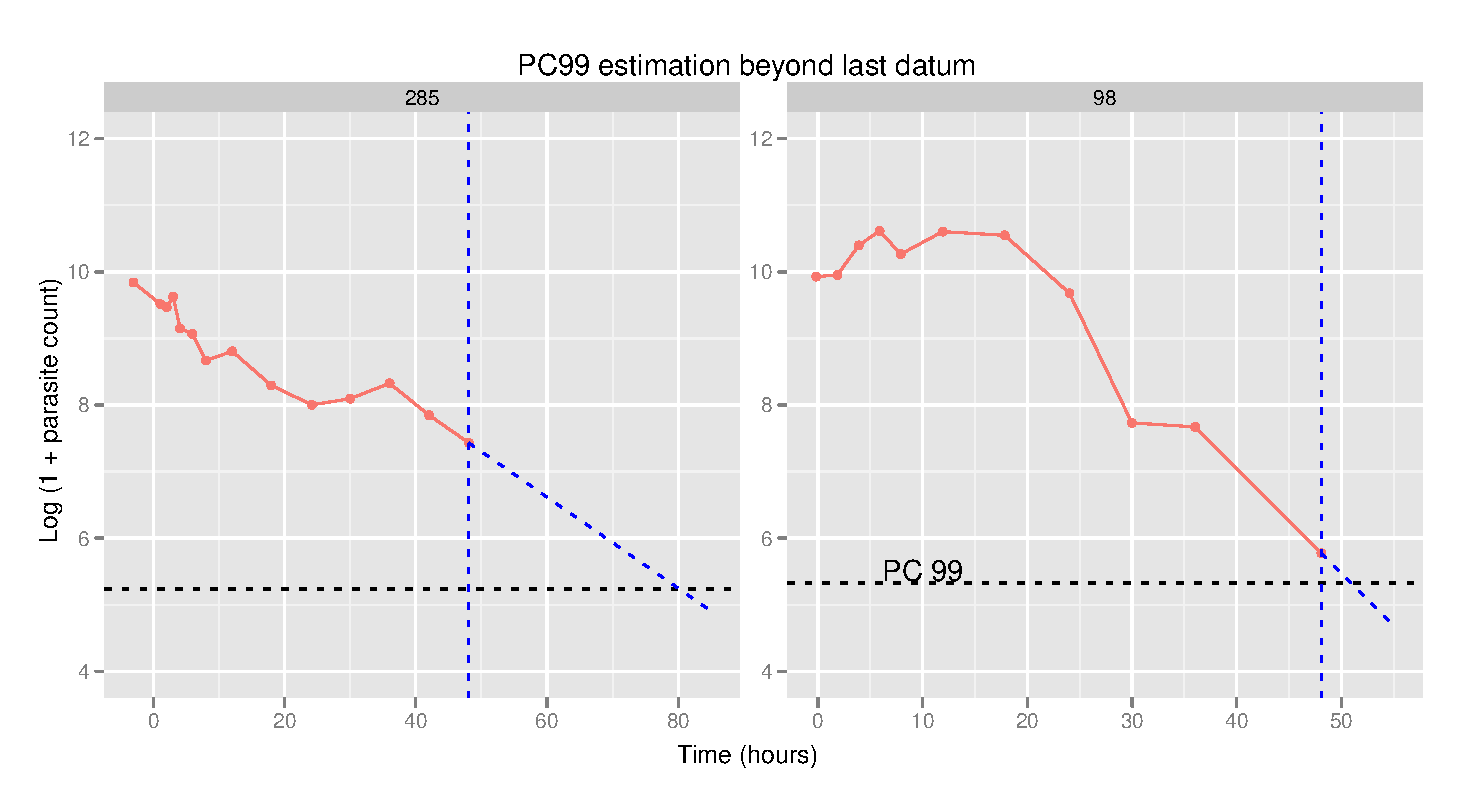
\includegraphics[width=150mm]{pc99extrap.eps} 
\caption{Bounds for PC99 estimates based between immediate cut-off and linear extrapolation}
\label{pc99extrap}
\end{figure}
We define an upper estimate for PC99 as that predicted by linear extrapolation and a lower estimate simply assumes that the parasite count dropped below PC99 immediately after the last reading.

For subject 477 the parasite count drops below PC99 but then rises again as shown in Figure \ref{477}.
\begin{figure}[h]
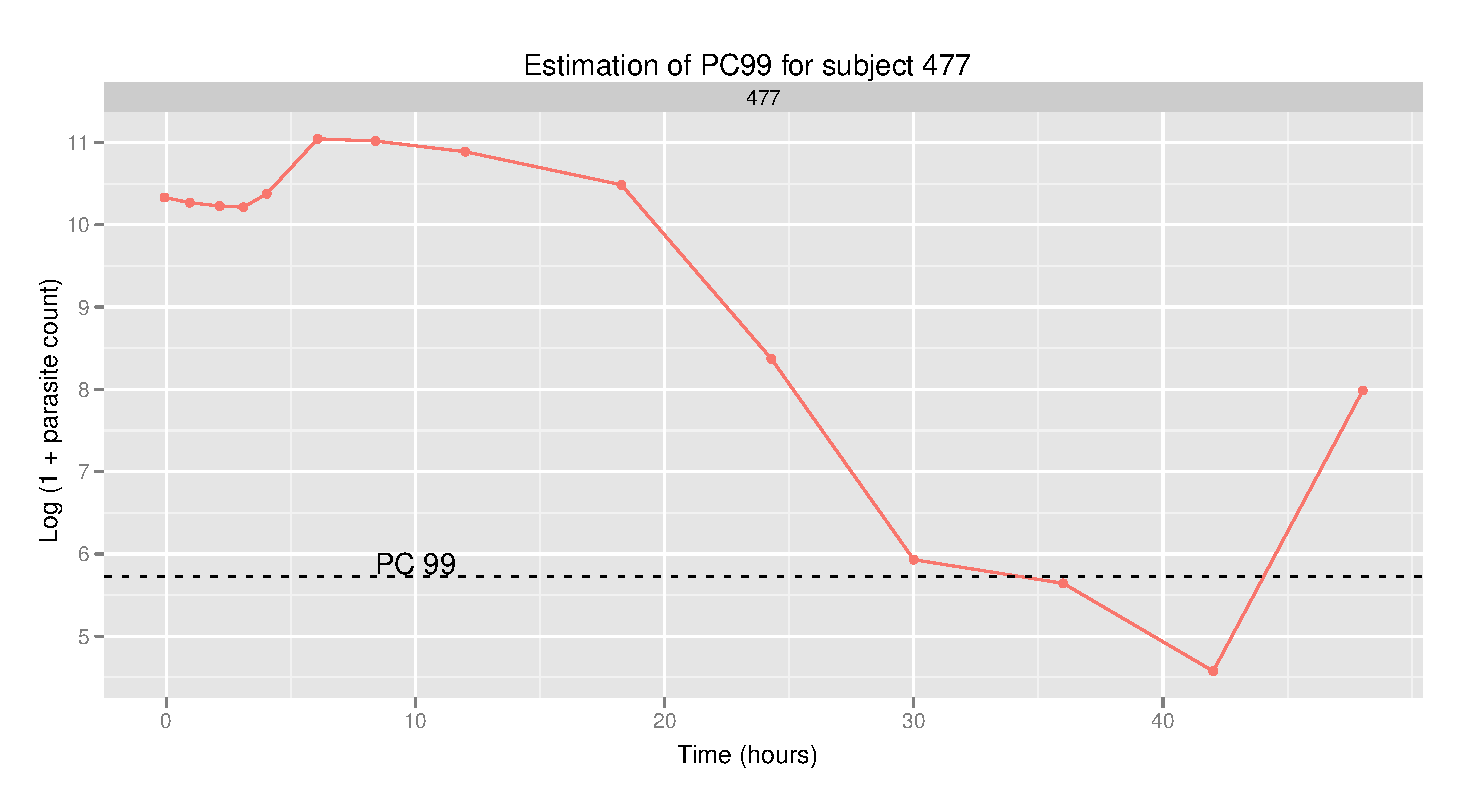
\includegraphics[width=150mm]{477.eps} 
\caption{PC99 estimation for subject 477}
\label{477}
\end{figure}
In this case we can take the lower bound for the estimate as the first time the PC99 is reached, thereby assuming that the last datum is a false reading. It is not clear what to use as the upper estimate, but a starting point is to set it equal to the largest PC99 value observed.

%Once again there is no discernible effect of centre or sex alone on the clearance times. However, now the improvement of the combined treatment over the single treatment seems more symmetrical between sexes.
Results of 2-way ANOVA by sex and treatment on the square-root transformed clearance times fitted by treatment-weighted least-squares are shown in Tables \ref{aov99low} and \ref{aov99high} using the lower and upper estimates respectively for PC99 for the 2 subjects where PC99 was not reached and subject 477 where the parasite count rose again after PC99.
%              Df Sum Sq Mean Sq F value    Pr(>F)    
%Sex            1  0.926   0.926  0.8609 0.3591839    
%Treatment      1 15.809  15.809 14.7031 0.0004477 ***
%Sex:Treatment  1  2.228   2.228  2.0720 0.1580030    
%Residuals     39 41.934   1.075            
\begin{table}[h]
\centering
\caption{ANOVA table for PC99 model with lower estimates for missing data}\label{aov99low}
\begin{tabular}{l|rrrrrl}
Source&Sum Sq.&df&Mean Sq.&$F$&P($>F$)\\
\hline
$Sex$				& 0.926 & 1 & 0.926 & 0.861 & 0.359 & \\
$Treatment$			& 15.81   & 1 & 15.81   & 14.70   & 0.0004 &*** \\
$Sex\times Treatment$	& 2.23   & 1 & 2.23   & 2.07   & 0.158 & \\
$Residuals$			& 41.93 & 39 & 1.08 &&&\\
\hline
Total&60.90&42&&&
\end{tabular}\\
***$<0.0005$
\end{table}

%              Df Sum Sq Mean Sq F value    Pr(>F)    
%Sex            1  0.216   0.216  0.1464 0.7040962    
%Treatment      1 22.011  22.011 14.8867 0.0004173 ***
%Sex:Treatment  1  4.736   4.736  3.2028 0.0812809 .  
%Residuals     39 57.665   1.479
\begin{table}[h]
\centering
\caption{ANOVA table for PC99 model with upper estimates for missing data}\label{aov99high}
\begin{tabular}{l|rrrrrl}
Source&Sum Sq.&df&Mean Sq.&$F$&P($>F$)\\
\hline
$Sex$				& 0.216 & 1 & 0.216 & 0.146 & 0.704 & \\
$Treatment$			& 22.01   & 1 & 22.01   & 14.89   & 0.0004 &*** \\
$Sex\times Treatment$	& 4.74   & 1 & 4.74   & 3.20   & 0.081 & \\
$Residuals$			& 57.67 & 39 & 1.48 &&&\\
\hline
Total&60.90&42&&&
\end{tabular}\\
***$<0.0005$
\end{table}

It can be seen that there is good evidence to reject the hypothesis that treatment has no effect on PC99 clearance time, but no evidence to reject the hypothesis that sex has no effect. Raising the upper estimate of subject 477 to over 100 does not alter the outcome of the hypothesis tests. Since subject 477 is male and the other two subjects for whom an extrapolated PC99 estimates were made are female, the ANOVA was repeated with the high and low estimates set opposite between sexes. This did not alter the outcome of the hypothesis tests.

If we average over both lower and upper estimates for the missing data, this gives a reduction in PC99 for subjects on the combined treatment of 12.1 hours with a 95\% confidence interval of (7.5, 16.9) hours.
%Therefore, we can exclude sex as a factor and refit a 1-way ANOVA model by treatment alone, giving the results shown in Table \ref{aov99r}.
%%            Df Sum Sq Mean Sq F value  Pr(>F)   
%%Treatment    1  9.396   9.396  9.3959 0.00399 **
%%Residuals   38 38.000   1.000   
%\begin{table}[h]
%\centering
%\caption{1-way ANOVA table for PC99 model}\label{aov99r}
%\begin{tabular}{l|rrrrrl}
%Source&Sum Sq.&df&Mean Sq.&$F$&P($>F$)\\
%\hline
%$Treatment$			& 9.40   & 1 & 9.40   & 9.40   & 0.004 &** \\
%$Residuals$			& 38.0 & 38 & 1.00 &&&\\
%\hline
%Total&47.40&39&&&
%\end{tabular}\\
%**$<0.005$
%\end{table}

%The mean PC99 clearance time for patients on the single treatment is 21:07 (hrs:mins) with a 95\% confidence interval of (16:12, 26:41); for the combined treatment it is 12:33 (9:53, 15:32). This gives a mean decrease in PC99 for subjects on the combined treatment over the single treatment of 9.3 hours with a 95\% confidence interval of (3.7, 15.0) hours.

%\subsubsection{Survival analysis}
%An alternative method to handle the effectively \emph{right-censored} PC99 times is to use survival analysis techniques. If we define an ``event'' as the parasite count being reduced by 99\% then we have a set of ``survival'' times up to the occurrence of our event of interest with 3 right-censored times at 48 hours.



\subsection{Parasite reduction ratios}
Another endpoint used in studies of the efficacy of antimalarial drugs is the \emph{Parasite Reduction Ratio}, which is the ratio of the pre-dose parasite count to the count at a specific time from the time of first dose. 48 hours is often chosen as a time to calculate this ratio (PRR$_{48}$) as this represents the reduction in parasites over a single life-cycle of the parasites \cite{white}. ``PRR$_{24}$'', The reduction over 24 hours is also used \cite{newton}.

PRR48 measurements are not available for our data as the parasite count is 0 by 48 hours for all but 6 subjects. After 24 hours there are only 25 of the 43 subjects with non-zero parasite counts. Even after 12 hours there are only 37 of the 43 subjects with a non-zero parasite counts. Consequently, it was decided that analysis of parasite reduction ratios was not suitable for this data.

An alternative, but similar approach is to look at the ratio of the count at a specific time to the pre-dose count, which is effectively 1/PRR. This has already been looked at in section \ref{sec:develt} and is studied further in the next section on functional data analysis.
%so we can look at PRR12 and have reasonable numbers in groups to make comparisons between treatments. The log parasite reduction ratio after 12 hours is shown in Figure \ref{prr12}
%\begin{figure}
%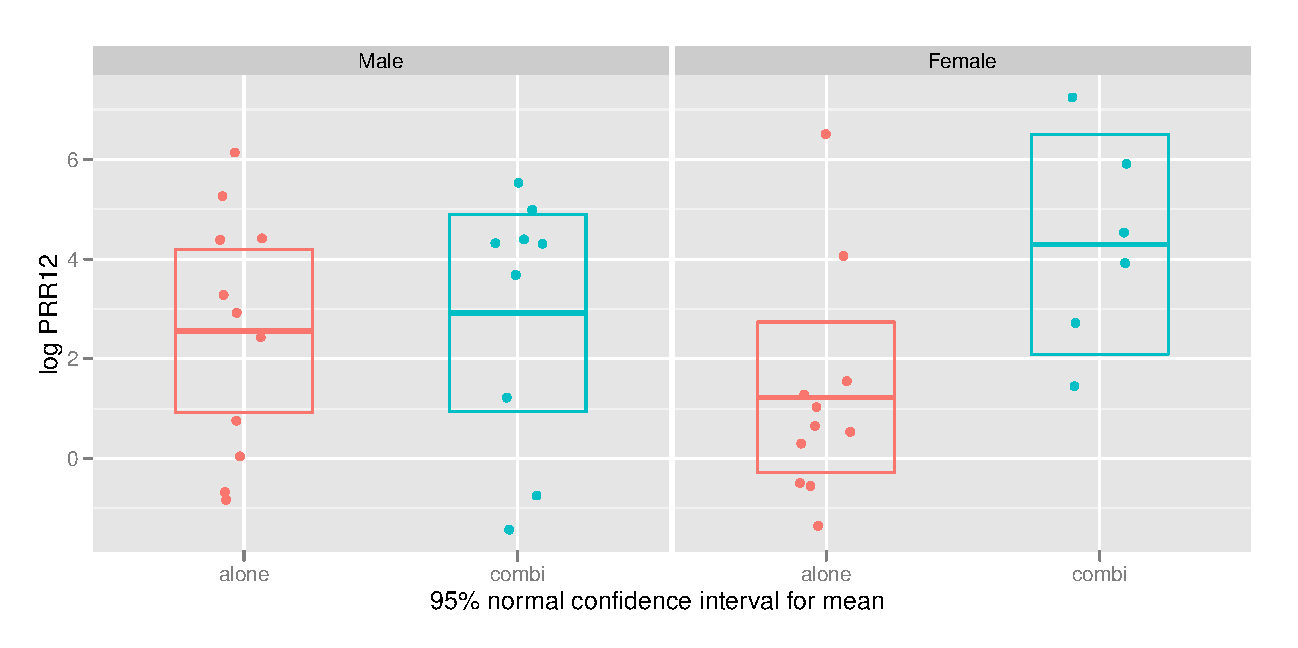
\includegraphics[width=150mm]{prr12.eps} 
%\caption{log PRR12 with 95\% confidence intervals for the means}
%\label{prr12}
%\end{figure}

%A similar pattern as with the PC90 and PC50 endpoints can be seen in that the treatment only seems to be effective among female patients in increasing PRR. It was found that a logarithmic transformation was appropriate for 2-way ANOVA modelling of the PRR12 data giving the results shown in Table \ref{aovprr12}.
%%              Df  Sum Sq Mean Sq F value  Pr(>F)  
%%Sex            1   1.524   1.524  0.2725 0.60512  
%%Treatment      1  21.265  21.265  3.8024 0.05972 .
%%Sex:Treatment  1  15.951  15.951  2.8521 0.10069  
%%Residuals     33 184.557   5.593          
%\begin{table}[h]
%\centering
%\caption{ANOVA table for PC99 model}\label{aovprr12}
%\begin{tabular}{l|rrrrrl}
%Source&Sum Sq.&df&Mean Sq.&$F$&P($>F$)\\
%\hline
%$Sex$				& 1.52 & 1 & 1.52 & 0.273 & 0.605 & \\
%$Treatment$			& 21.27   & 1 & 21.27   & 3.80 & 0.060 & \\
%$Sex\times Treatment$	& 15.95   & 1 & 15.95   & 2.85   & 0.101 & \\
%$Residuals$			& 184.56 & 33 & 5.59 &&&\\
%\hline
%Total&223.30&36&&&
%\end{tabular}
%\end{table}

%It can be seen that there is some evidence between the 5 and 10\% level to reject the hypothesis that the treatment has no effect on the parasite reduction ratio after 12 hours. It may be that we don't have enough data to detect the treatment effect observed in Figure \ref{prr12}. The model gives a mean increase in PRR12 for subjects on the combined treatment over those on the single treatment of 25.5 with a 95\% confidence interval of (-0.4, 159.8).

%\subsection{Logistic model of those cured after 24 hours?}

\section{Functional data analysis}
\subsection{Overview of functional data analysis}
Functional data analysis (FDA) is a relatively new technique whereby the data is analysed in terms of smooth functions. An example is longitudinal data such as the growth of children or the weather over a year \cite{ramsay}. With such data we describe the response with a smooth function and then look at the ways the characteristics of the function change between cases. For example, this type of analysis can make use of derivatives of the functions to look for patterns in rates of change. Functional data analysis is somewhat analogous to multivariate data analysis, looking at multiple responses and characteristic combinations of responses between cases.

The parasite count data in this study is a good candidate for functional data analysis in that the response for each replicate of experimental factors centre, sex and treatment can be described as a smooth function of parasite count with time. We already used cubic and logistic functions in order to extract a single response variable, the PC90 clearance time, but now we can go on to explore the nature of a functional response.

Many familiar statistical summaries and techniques have functional equivalents. Means and standard deviations can be expressed as mean functions and standard deviation functions for example. Regression and ANOVA can be performed with functional dependent and independent variables yielding residual, $F$ statistic and coefficient functions.

\subsection{Basis functions}
The first step in FDA is to identify an appropriate smoothing function for our data known as a \emph{basis function}. For periodic data fourier functions are normally used, for non-periodic data the most commonly used basis functions are cubic splines \cite{fdaweb}. Fitting a cubic spline requires choice of \emph{breakpoints} between which we fit cubic polynomials. The simplest choice of breakpoints with longitudinal data is to choose the times at which the data were taken. We also specify a smoothness parameter that limits the size of higher derivatives and hence the sharpness of the curve.

\subsubsection*{Fitting a basis function to the parasite count data}
We want to compare the development of parasite count with time between subjects using a scale that is independent of the absolute count. Hence we will use the fraction of the pre-dose parasite count. We determined that a logarithmic transform of the count is appropriate for this data and hence we will use as our time-dependent variable $y(t)$
$$y(t)=\log (1+P(t))-\log(1+P_{0})$$
which is the logarithm of the ratio of the parasite count at time $t$, $P(t)$, to the pre-dose parasite count $P_{0}$. 1 is added to both so that the logarithm of 0 count is 0.

Ramsay \textit{et al.} have written a \emph{R} package, \texttt{fda} \cite{fdaR, fdaRbook} for functional data analysis. The functions in this package were used to fit cubic splines to the data. The level of smoothing is determined by penalising derivatives of the spline function. It was found that penalising the 2nd derivative (the rate of change of slope) by a factor of 10 gave reasonable smoothing such that the fitted curves were insensitive to small-scale (perhaps random-error scale) variation but described the overall trend of the parasite count well. The resulting curves for the 43 subjects are shown in Figure \ref{cubicspline}.
\begin{figure}[h]
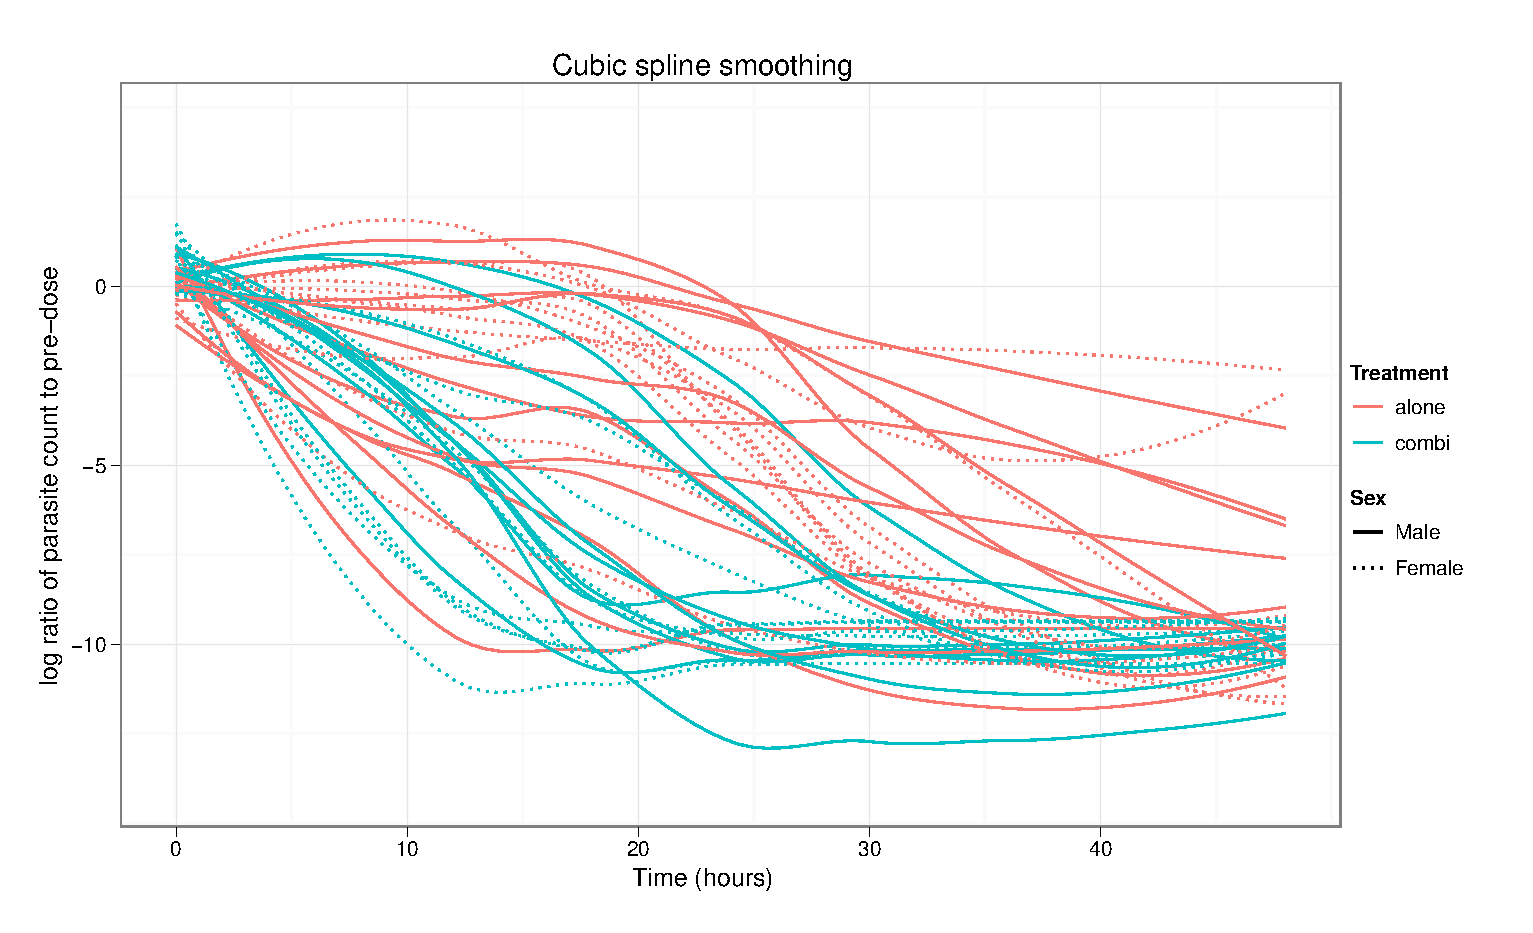
\includegraphics[width=150mm]{cubicspline.eps} 
\caption{Cubic splines fitted to the parasite count, smoothed by penalising the 2nd derivative}
\label{cubicspline}
\end{figure}

\subsection{Functional ANOVA}
Once we have suitably represented our dependent data as a functional response we can perform ANOVA by sex and treatment in an analogous way to the previous analyses. The model now becomes
\begin{equation}
y_{jkl}(t)=\mu(t)+S_{j}(t)+T_{k}(t)+(ST)_{jk}(t)+\epsilon_{jkl}(t)\quad\quad\epsilon\sim N(0, \sigma^{2}(t))\label{aovfda}
\end{equation}
where each part of the model is now a function of time. Hence, we will have 43 residual functions, a mean function for the overall mean with time, $\mu(t)$, a function for the effect of sex, $S(t)$, and for the effect of treatment, $T(t)$.

The standardized residuals ($e_{jkl}(t)/\hat{\sigma}(t)$) from fitting this model are shown in Figures \ref{fdaresids} and \ref{fdahistqq}. It can be seen that they are approximately normally distributed about 0 indicating that our parameter function estimates will be unbiased.
\begin{figure}[p]
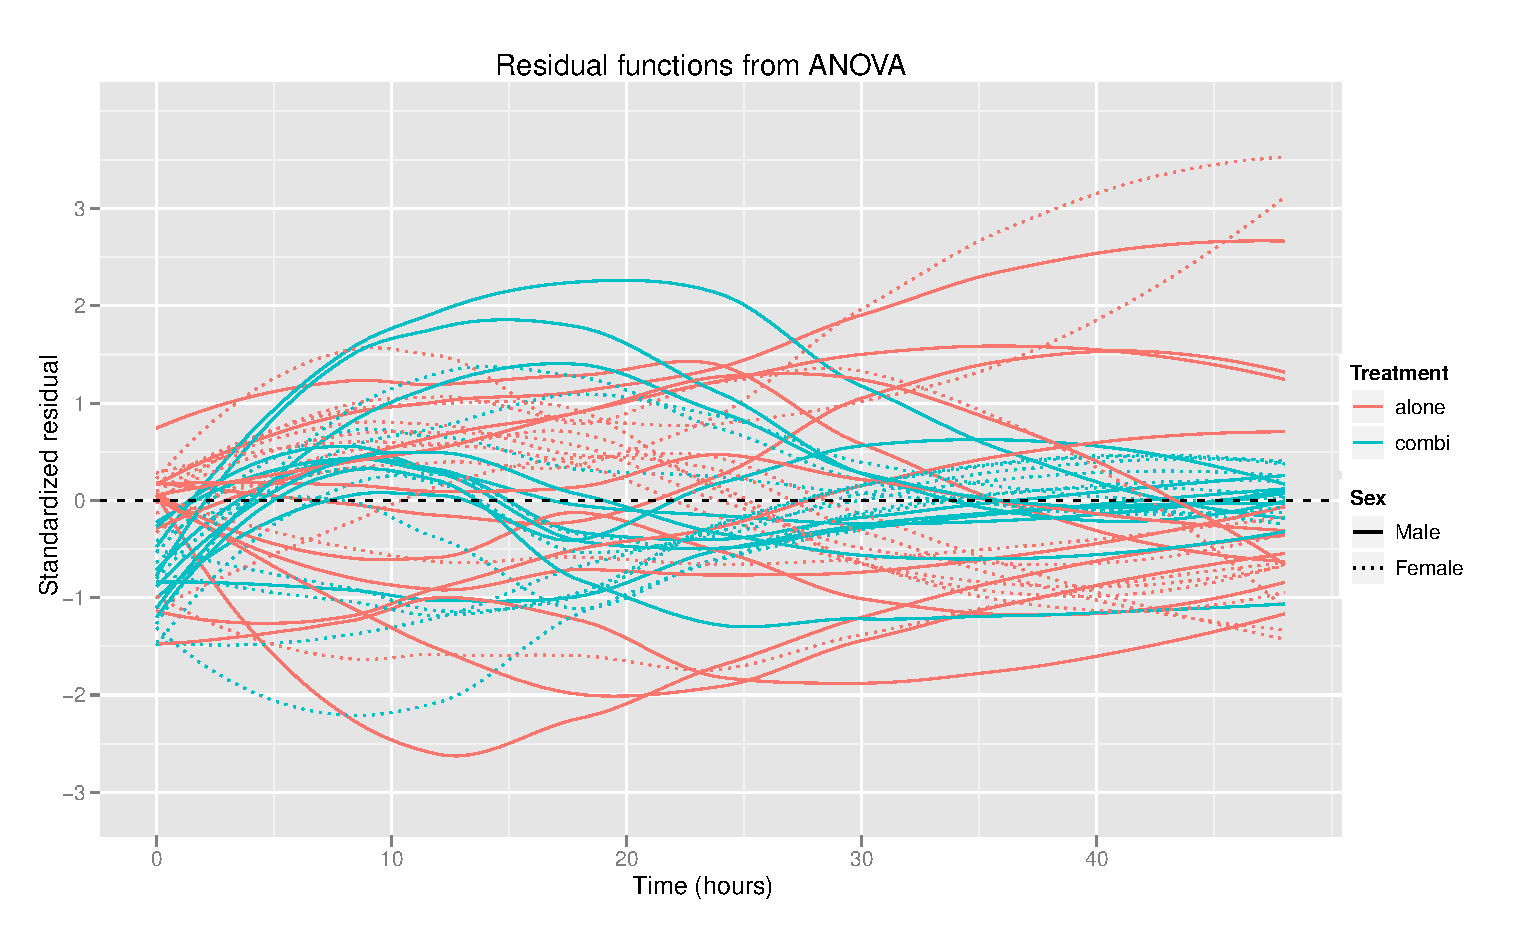
\includegraphics[width=150mm]{fdaresids.eps} 
\caption{Standardized residual functions for 2-way functional ANOVA}
\label{fdaresids}
\end{figure}
\begin{figure}[p]
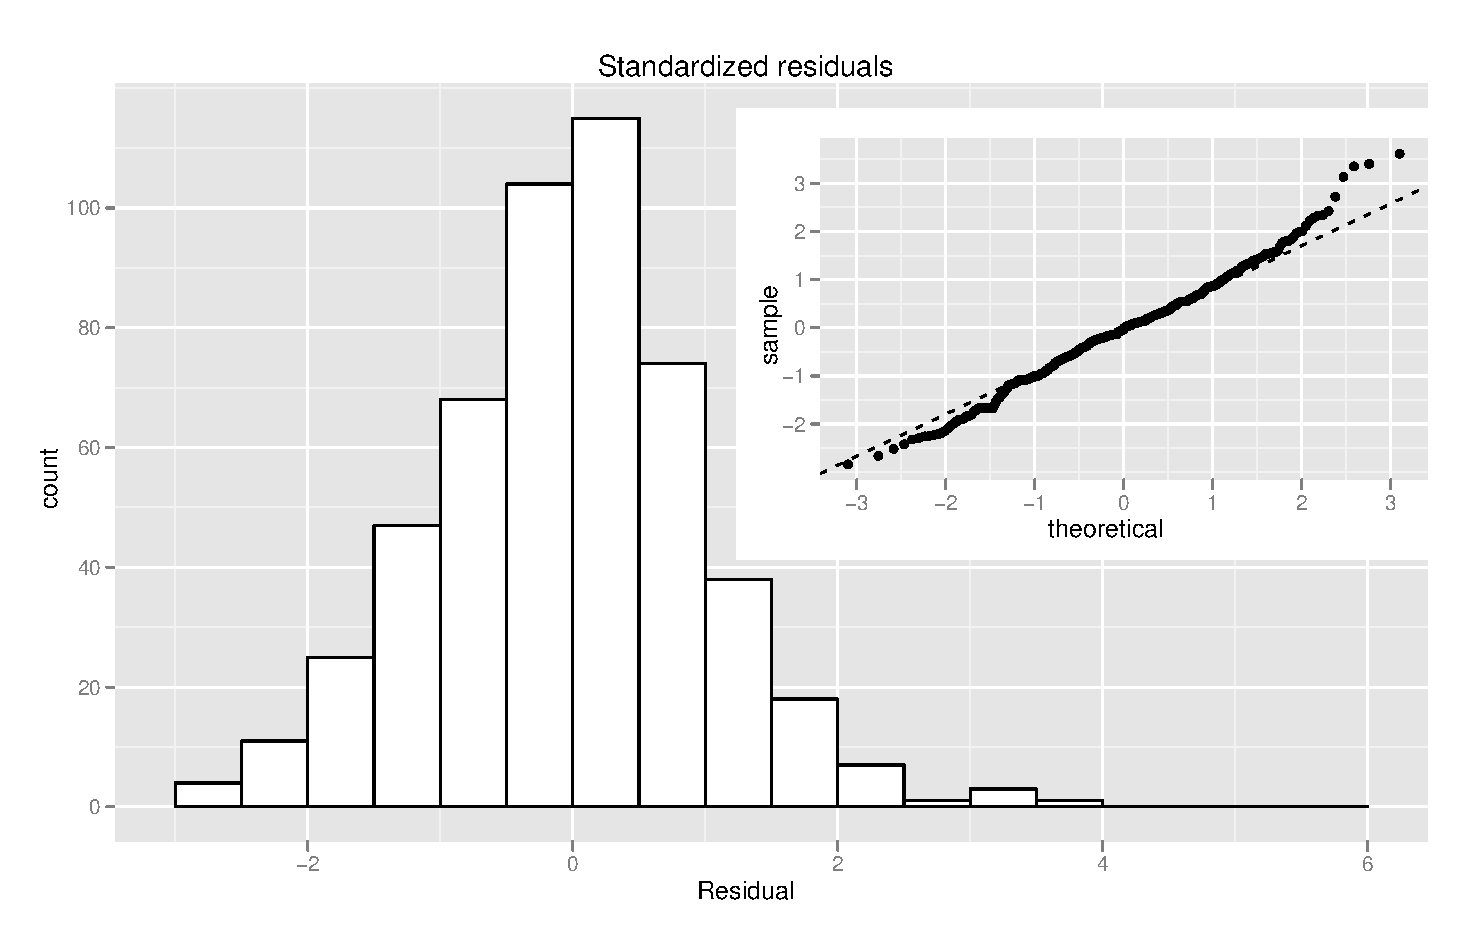
\includegraphics[width=150mm]{fdahistqq.eps} 
\caption{Distribution of standardized residuals for 2-way functional ANOVA}
\label{fdahistqq}
\end{figure}

The \texttt{fda} library provides functions for deriving a permutation $F$ test similar to the methods used in section \ref{section:resampling}. The results of this permutation $F$ test for our 2-way ANOVA are shown in Figure \ref{fdapermF}. The pointwise critical value is relevant if we look at any one time, but for making simultaneous hypothesis tests over all times we should use the maximum critical value shown. It can be seen that the null hypothesis of no difference of sex or treatment groups is not rejected up to 10 hours from first dose, then there is evidence after 10 hours to reject the null hypothesis, with no evidence for rejection after about 30 hours. This can be explained by the parasite count being independent of sex and treatment allocation at the start, with significant differences in the count trajectories developing between the groups as time goes on, with them eventually returning to parity as clearance is finally achieved for all subjects.
\begin{figure}[p]
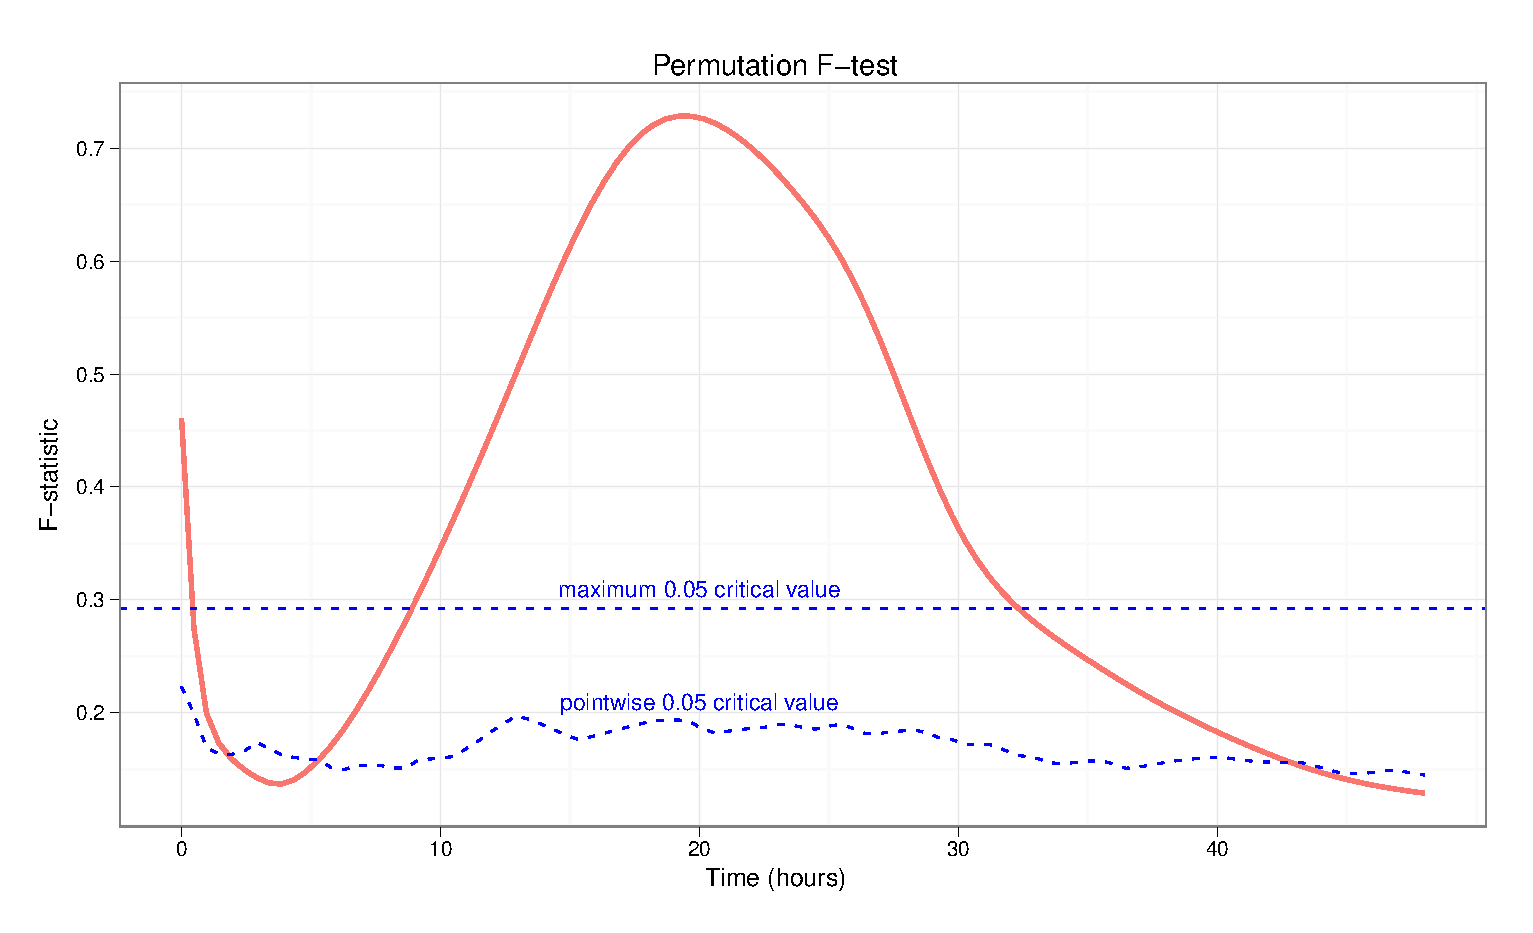
\includegraphics[width=150mm]{fdapermF.eps} 
\caption{$F$ statistic function for 2-way functional ANOVA. The critical value at each time is shown and the critical value for the maximum $F$ statistic over all times.}
\label{fdapermF}
\end{figure}

Figure \ref{fdcoef} shows the fitted coefficient functions.
\begin{figure}[p]
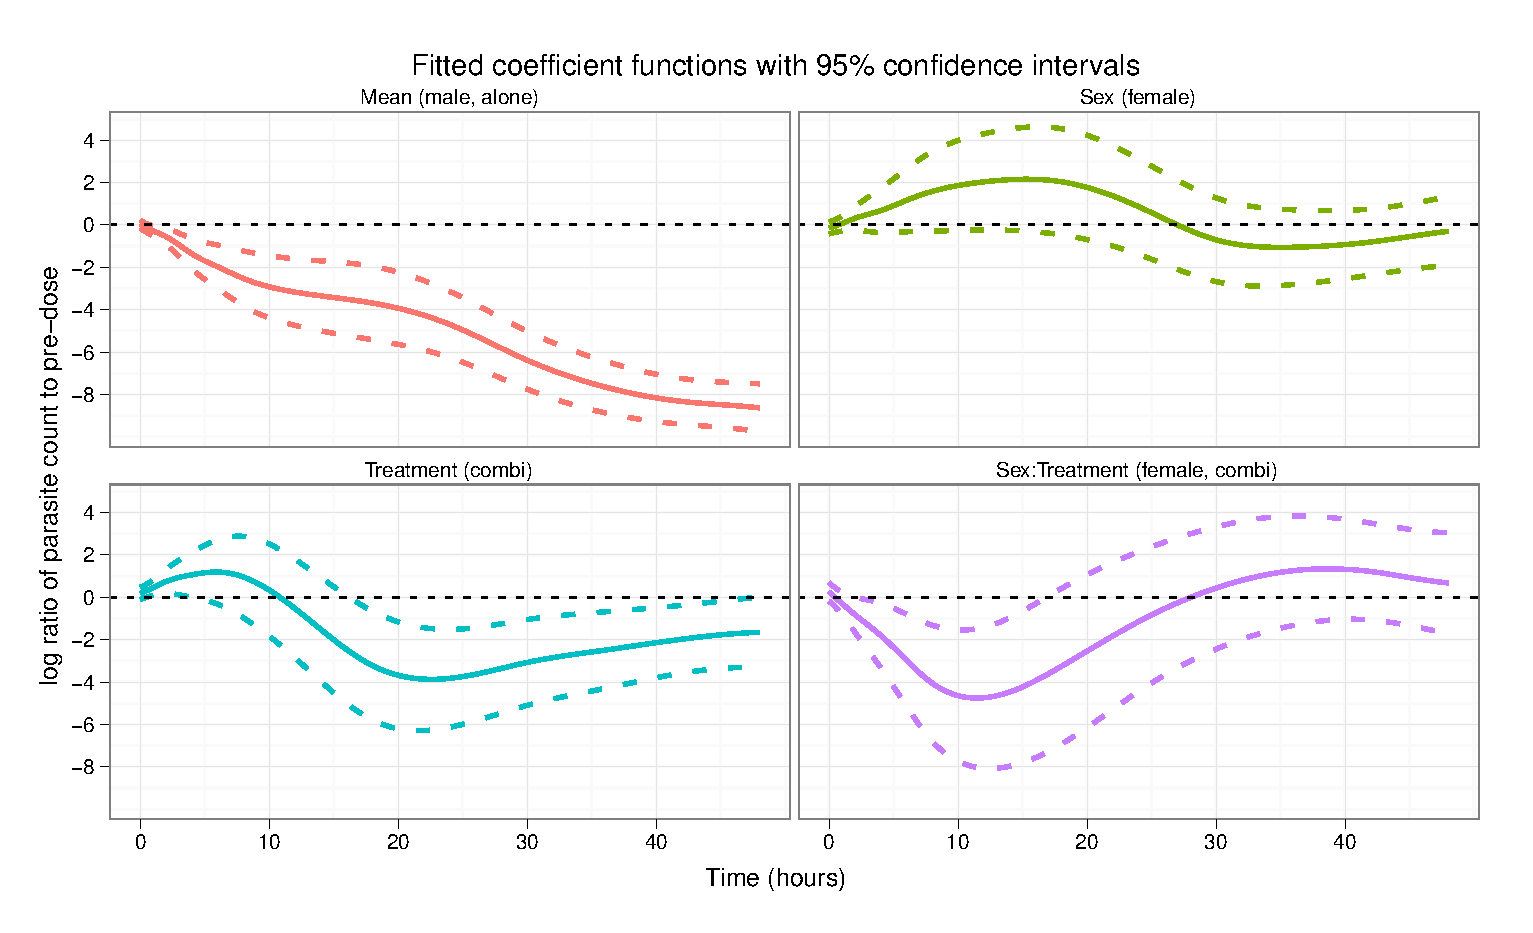
\includegraphics[width=150mm]{fdcoef.eps} 
\caption{Fitted coefficient functions for 2-way ANOVA model \ref{aovfda} (page \pageref{aovfda}). From top-left, to bottom-right, the functions are $\mu(t)$, $S(t)$, $T(t)$, $ST(t)$.}
\label{fdcoef}
\end{figure}
 The top-left panel shows the mean $\mu$ corresponding to male subjects on the single treatment with the other panels showing the deviation from this mean due to sex, treatment and the interaction of sex and treatment respectively. We can see that there is no evidence at the 5\% level over the whole time period to reject the hypothesis that sex has no effect. Between approximately 17 and 45 hours there is evidence to reject the hypothesis that treatment has no effect and between 10 and 15 hours there is evidence to reject the hypothesis that there is no interaction between sex and treatment that effects the parasite count.
 
Figure \ref{fdfitted} shows the fitted mean-level functions with 95\% confidence intervals\footnote{The routines for calculating the standard errors and confidence intervals of predicted functions are not yet implemented in the \emph{R} \texttt{fda} library, hence it was necessary to implement these (Listing \ref{R:fdaresid} in Appendix \ref{A:fda}).}.
\begin{figure}[p]
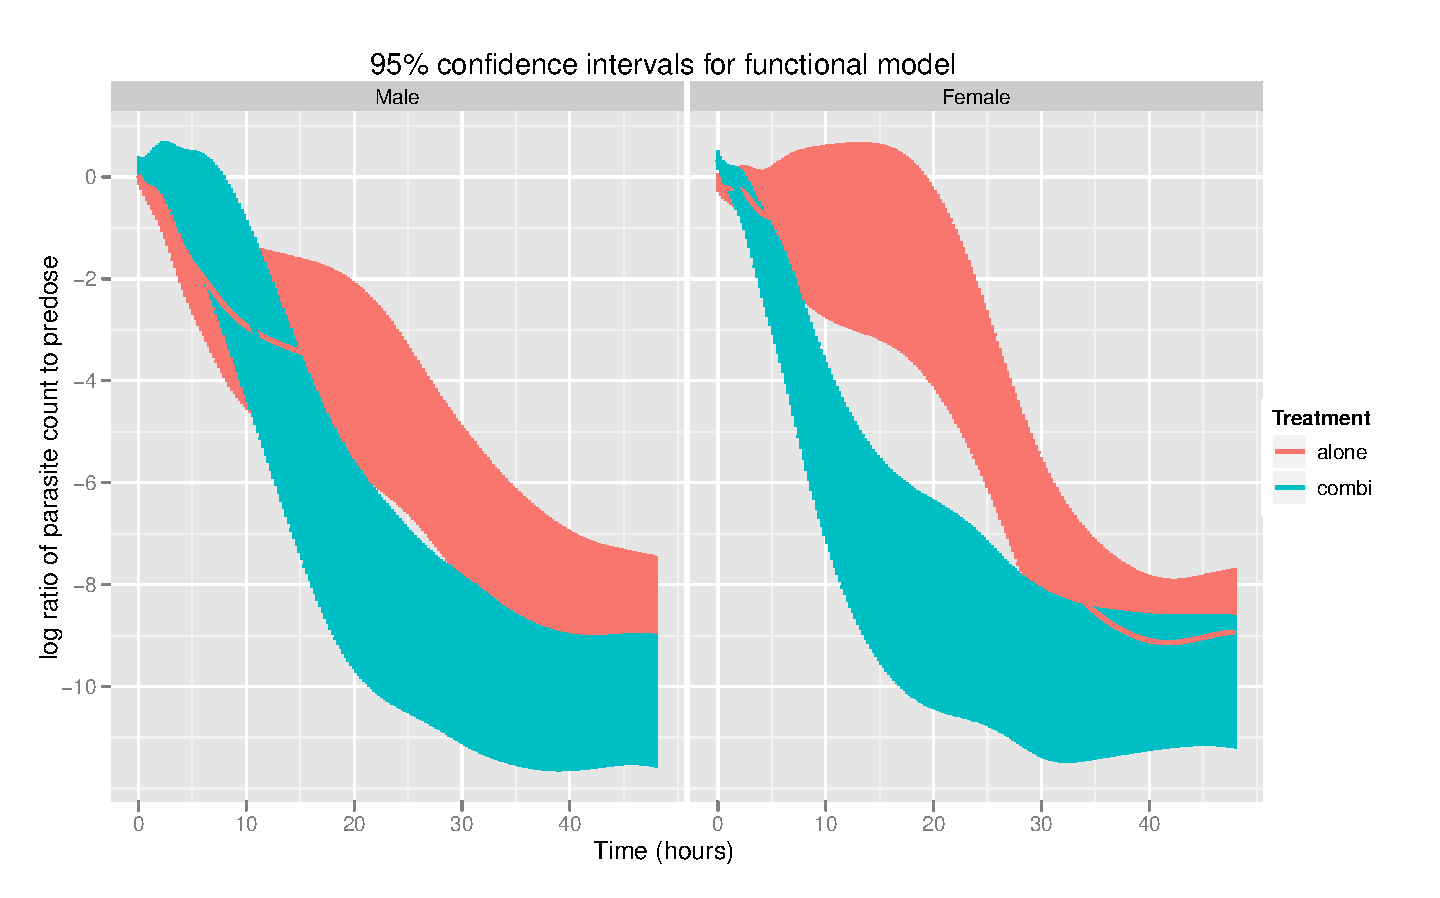
\includegraphics[width=150mm]{lprr2i.eps} 
\caption{Fitted count-ratio functions with confidence intervals}
\label{fdfitted}
\end{figure}
It can be seen that the difference between male subjects on the alone and combined drug treatment becomes large (relative to their 95\% confidence limits) between 20 and 30 hours reflecting the treatment effect shown in Figure \ref{fdcoef} between 20 and 30 hours. The difference between treatments for female subjects is larger between 10 and 30 hours reflecting the combined effect of treatment and the sex-treatment interaction: the effect is essentially an addition of the bottom two panels in Figure \ref{fdcoef}. With reference to the 95\% confidence intervals, there is good evidence to reject the hypothesis that there is no effect of sex and treatment. The $F$ test in Figure \ref{fdapermF} is a more formal evaluation of this evidence.

If we look again at Figure \ref{fdfitted}, we can see that although the parasite reduction is comparable (confidence intervals almost fully overlapped) between treatments for male subjects, it is clear that the profiles have very different slopes between treatments; similarly for female patients, although the actual reduction level is also different. With functional data analysis it is easy to look, not only at the effect of factors on the dependent variable function, but also at the effect on derivatives of the response function. Accordingly, the functional ANOVA was repeated, but this time with the first derivative of the log count-ratio cubic spline functions. This fitted model is shown in Figure \ref{fdspeed}. 
\begin{figure}[p]
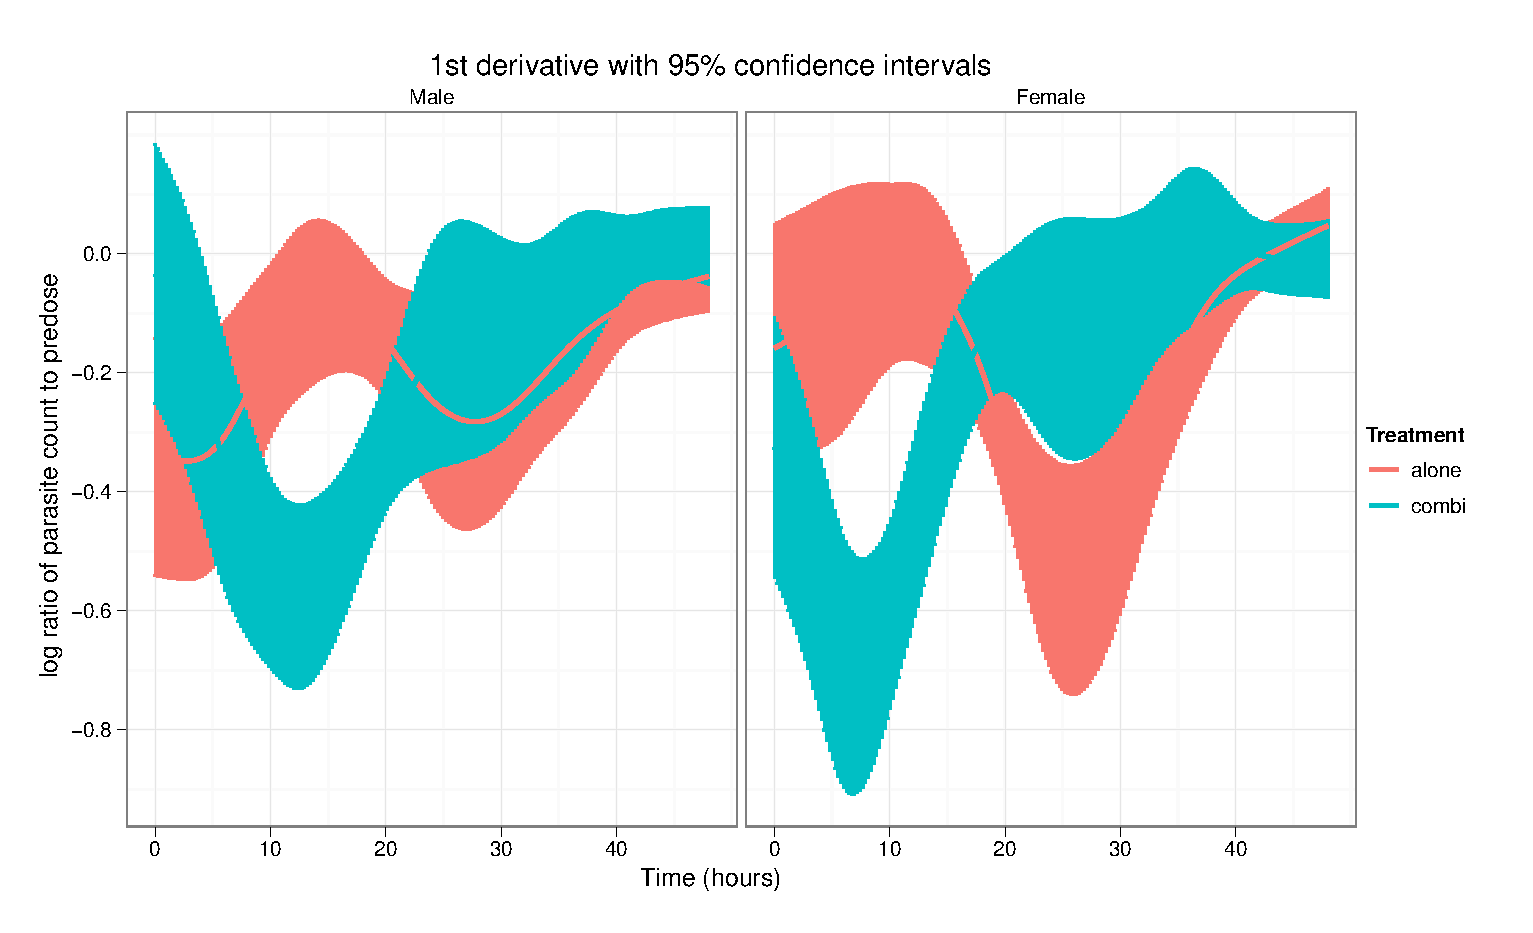
\includegraphics[width=150mm]{lprr2ispeed.eps} 
\caption{Fitted functional model for 1st derivative of count ratio showing the effect of treatment on the instantaneous \emph{speed} of parasite clearance}
\label{fdspeed}
\end{figure}

It can be seen that the initial \emph{speed} of reduction is significantly faster (larger negative magnitude) from 10 to 15 hours for the combined treatment for both sexes, whereas the level of reduction (Figure \ref{fdfitted}) is not significantly different for male subjects up to at least 20 hours. What we can see from Figure \ref{fdspeed} is that the parasite-killing effect doesn't ``kick in'' and reach its maximum speed of parasite reduction until around 25 hours from first dose for the alone treatment, as opposed to around 10 hours for the combined treatment.
\clearpage
\section{Key results}
In this chapter some alternative methods of looking at how the parasite clearance is affected by experimental factors were explored. The key findings are:
\begin{itemize}
\item There is marginal evidence ($0.05<p<0.1$) to reject the hypothesis that there is no effect of a sex-treatment interaction on the time for half the parasites to be cleared from the blood (PC50). The reduction in PC50 clearance time for female patients on the combined treatment over the single treatment is 7.1 hours with a 95\% confidence interval of (0.7, 9.9) hours. There is no evidence to reject the hypothesis that PC50 clearance times are the same for male subjects on either treatment.
\item There is good evidence ($p<0.0005$) to reject the hypothesis that treatment has no effect on the time for 99\% of parasites to be cleared from the blood (PC99). The result of this hypothesis test is not altered when lower and upper extreme estimates are made for 3 subjects for whom PC99 was not obtained within the time period of the trial. The reduction in PC99 for subjects on the combined treatment is 12.1 hours with a 95\% confidence interval of (7.5, 16.9) hours.
\item The technique of functional data analysis was applied to this data whereby the parasite count profiles are described by smooth cubic-spline functions. The functional equivalent of ANOVA was then performed on these splines by sex and treatment. This gave evidence to reject the hypothesis that treatment has no effect on the parasite count between 17 and 45 hours from first dose and evidence to reject the hypothesis that there is no interaction between sex and treatment that affects the parasite count between 10 and 15 hours.
\item The maximum speed of parasite reduction is obtained for the combined treatment around 15 hours before the single treatment.
\end{itemize}